\chapter{Transition Metals and Coordination Complexes}\label{ch:b2:coordination-complexes}

In 1893 a chemist of twenty-six, Alfred Werner, set out to explain a puzzle.
Cobalt(III) chloride forms four compounds with ammonia, \ce{CoCl3.6NH3},
\ce{CoCl3.5NH3} and two of formula \ce{CoCl3.4NH3}, one green and one violet.
Silver nitrate precipitates all three chlorides of the first at once, two of
the second, and only one of each of the last two. Werner's answer --- six
groups held around the metal at the corners of an octahedron, the rest outside
--- founded coordination chemistry. This chapter extends the complexes of the
Year 1 volume to their geometry, their isomers, their names, and a count of
electrons that predicts which metal carbonyls exist.

\begin{recall}
The Year 1 volume: complex, central atom, ligand, polydentate ligand, chelate,
formation constants, coordination number; electron configurations of the
transition-metal ions (the $n$s electrons lost first); Lewis acids and bases,
dative bonds; VSEPR; oxidation numbers; enantiomers. \Cref{ch:b2:atomic-orbitals}:
the d orbitals and the order of the 4s and 3d levels.
\end{recall}

\begin{omfigure}
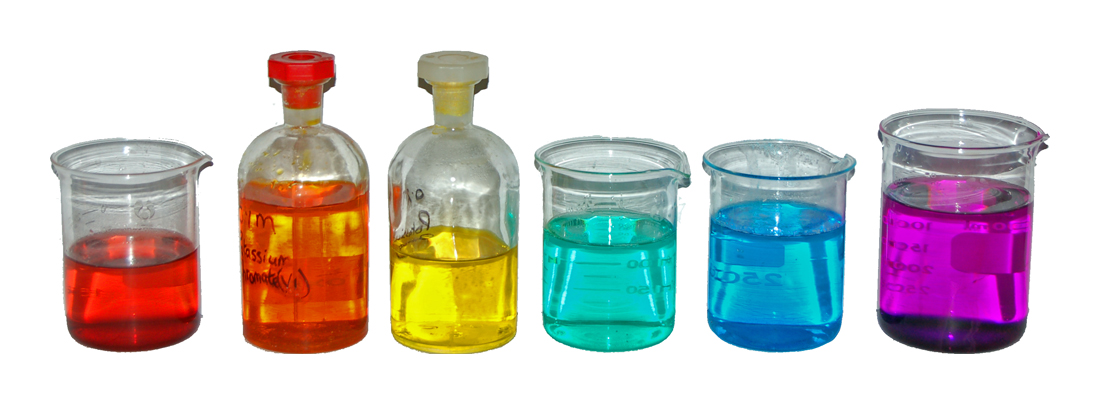
\includegraphics[width=0.8\linewidth]{images/book3/tm-solutions.jpg}

{\small Aqueous solutions of transition-metal compounds: from left to right,
cobalt(II) nitrate, potassium dichromate, potassium chromate, nickel(II) chloride,
copper(II) sulfate and potassium permanganate. The colours of the cobalt, nickel
and copper solutions come from their aqua complexes. (Photograph: Benjah-bmm27,
public domain, Wikimedia Commons.)}
\end{omfigure}

\section{The d block}

\begin{definition}[Transition element]\label{def:b2:coordination-complexes:transition-element}
A \emph{transition element}\index{transition element} is an element whose atom, or
one of whose common ions, has a partly filled d subshell. An ion of such an element
with $n$ electrons in its d orbitals has a \emph{$d^n$ configuration}\index{dn
configuration@$d^n$ configuration}.
\end{definition}

\begin{proposition}[Counting d electrons]\label{prop:b2:coordination-complexes:dn}
A transition-metal ion $\mathrm M^{m+}$ of the group numbered $g$ (3 to 12) has a $d^n$
configuration with $n = g - m$.
\end{proposition}

\begin{proof}
The neutral atom has $g$ electrons beyond the preceding noble gas, in the $n$s and
$(n - 1)$d orbitals. In the ions, the d orbitals lie below the s orbital
(\cref{ex:b2:atomic-orbitals:iron}): all the remaining $g - m$ valence electrons are d
electrons.
\end{proof}

For example \ce{Fe^2+} (group 8) is $d^6$, \ce{Cu^2+} (group 11) $d^9$, \ce{Co^3+} (group 9)
$d^6$, \ce{Pt^2+} (group 10) $d^8$.

\section{Ligands}

\begin{definition}[Denticity]\label{def:b2:coordination-complexes:denticity}
The \emph{denticity}\index{denticity} of a ligand is the number of its atoms bound to
the same central atom. A \emph{monodentate ligand}\index{monodentate ligand} binds
through one atom (\ce{H2O}, \ce{NH3}, \ce{Cl-}, \ce{CO}), a \emph{bidentate
ligand}\index{bidentate ligand} through two (ethane-1,2-diamine, written en; the
ethanedioate ion, ox). A \emph{bridging ligand}\index{bridging ligand} binds to two
metal atoms at once. An \emph{ambidentate ligand}\index{ambidentate ligand} can bind
through either of two different atoms, such as the nitrite ion (through N or O) or
thiocyanate (through S or N).
\end{definition}

\begin{definition}[Coordination sphere]\label{def:b2:coordination-complexes:coordination-sphere}
The \emph{coordination sphere}\index{coordination sphere} of a complex is the set of
the central atom and the ligands bound to it, written within square brackets; ions
outside the brackets are counter-ions, not bound to the metal.
\end{definition}

\begin{omfigure}
\setchemfig{atom sep=2.2em}
\chemfig{M*5(-H_2N-CH_2-CH_2-NH_2-)}
\qquad
\chemfig{M*5(-O-(=O)-(=O)-O-)}
\qquad
\chemfig{N(-[:120]CH_2COO^{-})(-[:240]CH_2COO^{-})-CH_2-CH_2-N(-[:60]CH_2COO^{-})(-[:-60]CH_2COO^{-})}

\medskip
{\small Chelating ligands. Left: ethane-1,2-diamine (en), bidentate through its two
nitrogens. Middle: the ethanedioate ion (ox), bidentate through two oxygens. Right:
the edta anion, which wraps round a metal ion with its two nitrogens and four
carboxylate oxygens (hexadentate).}
\end{omfigure}

\section{Coordination numbers and geometries}

Two, four and six are the commonest coordination numbers. Silver(I) and gold(I) give
linear complexes (\ce{[Ag(NH3)2]+}); four ligands form a tetrahedron
(\ce{[CoCl4]^2-}, \ce{[Zn(NH3)4]^2+}) or a square (\ce{[PtCl4]^2-}, \ce{[Ni(CN)4]^2-});
five, a trigonal bipyramid (\ce{Fe(CO)5}); six, by far the most frequent, an
octahedron.

\begin{omfigure}
\begin{tikzpicture}[font=\small]
  \node[omligand] at (-0.8,0) {}; \node[omligand] at (0.8,0) {};
  \draw[thick, black!70] (-0.8,0) -- (0.8,0); \node[ommetal] at (0,0) {};
  \node at (0,-1.5) {linear, 2};
  \pic at (3,0) {omtetrahedron}; \node at (3,-1.5) {tetrahedral, 4};
  \pic at (6,0) {omsquareplanar}; \node at (6,-1.5) {square planar, 4};
  \pic at (9,0) {omtbp}; \node[align=center] at (9,-1.65) {trigonal\\ bipyramidal, 5};
  \pic at (12,0) {omoctahedron}; \node at (12,-1.5) {octahedral, 6};
\end{tikzpicture}

{\small The common coordination geometries (metal orange, ligands grey; dashed
bonds point behind the page).}
\end{omfigure}

VSEPR, which places electron pairs of the central atom as far apart as possible,
fails here: a $d^8$ ion such as \ce{Pt^2+} carries four pairs of d electrons and four
ligands, yet its complexes are square, not tetrahedral or octahedral. The
d electrons are not localised pairs pushing the ligands: their energies depend
on the geometry in a way the next chapter computes.

\begin{proposition}[Square-planar $d^8$]\label{prop:b2:coordination-complexes:square-planar}
Four-coordinate complexes of $d^8$ ions of the second and third transition series
(\ce{Pd^2+}, \ce{Pt^2+}, \ce{Au^3+}) are square planar.
\end{proposition}

\admitted

The explanation, the splitting of the d levels by the ligands, comes in
\cref{ch:b2:ligand-field}.

\section{Isomers}

\begin{definition}[Isomers of complexes]\label{def:b2:coordination-complexes:isomers}
In an octahedral complex $\mathrm{MA_3B_3}$, the \emph{fac isomer}\index{fac isomer} has
the three B ligands on one face of the octahedron, the \emph{mer
isomer}\index{mer isomer} on a meridian (three positions in a plane through the
metal). \emph{Linkage isomers}\index{linkage isomers} differ by the atom through which
an \omterm{def:b2:coordination-complexes:denticity}{ambidentate ligand} binds. \emph{Ionisation isomers}\index{ionisation isomers}
exchange a ligand with a counter-ion, giving different ions in solution.
\end{definition}

\begin{proposition}[Counting octahedral isomers]\label{prop:b2:coordination-complexes:isomer-count}
In an octahedron, $\mathrm{MA_4B_2}$ has two isomers (cis and trans), $\mathrm{MA_3B_3}$ two
(fac and mer), and $\mathrm M(\mathrm{AA})_3$, with three \omterm{def:b2:coordination-complexes:denticity}{bidentate ligands}, two
enantiomers, $\Delta$ and $\Lambda$.
\end{proposition}

\begin{proof}
In an octahedron any two positions are either adjacent (cis, $90^\circ$) or opposite
(trans, $180^\circ$): two arrangements for the two B ligands. For three B ligands,
either no two are trans (they occupy one face: fac) or exactly one pair is trans (the
third is cis to both: mer); three mutually trans positions do not exist. For
$\mathrm M(\mathrm{AA})_3$, each chelate spans two cis positions; the three chelates
wind round the threefold axis as the blades of a propeller, turning either clockwise
or anticlockwise when viewed along that axis: two mirror images, not superimposable
since the complex has no mirror plane.
\end{proof}

\begin{omfigure}
\begin{tikzpicture}[font=\scriptsize]
  \pic (a) at (0,0) {omoctahedron};
  \node[omligand, fill=omDef!70] at (a-L1) {}; \node[omligand, fill=omDef!70] at (a-L3) {};
  \node at (0,-1.5) {\small cis-$\mathrm{MA_4B_2}$};
  \pic (b) at (3,0) {omoctahedron};
  \node[omligand, fill=omDef!70] at (b-L1) {}; \node[omligand, fill=omDef!70] at (b-L2) {};
  \node at (3,-1.5) {\small trans-$\mathrm{MA_4B_2}$};
  \pic (c) at (6.5,0) {omoctahedron};
  \node[omligand, fill=omThm!70] at (c-L1) {}; \node[omligand, fill=omThm!70] at (c-L3) {}; \node[omligand, fill=omThm!70] at (c-L5) {};
  \node at (6.5,-1.5) {\small fac-$\mathrm{MA_3B_3}$};
  \pic (d) at (9.5,0) {omoctahedron};
  \node[omligand, fill=omThm!70] at (d-L1) {}; \node[omligand, fill=omThm!70] at (d-L2) {}; \node[omligand, fill=omThm!70] at (d-L3) {};
  \node at (9.5,-1.5) {\small mer-$\mathrm{MA_3B_3}$};
\end{tikzpicture}

\medskip
\begin{tikzpicture}[font=\scriptsize]
  \foreach \xs/\s/\lab in {0/1/{$\Delta$}, 4.5/-1/{$\Lambda$}} {
    \begin{scope}[xshift=\xs cm, xscale=\s]
      \draw[black!30] (0,0) circle (1.2);
      \foreach \a in {90, 210, 330} {
        \coordinate (p) at (\a:1.1); \coordinate (q) at (\a+70:0.55);
        \draw[very thick, omDef] (\a:1.1) .. controls (\a+30:1.25) and (\a+60:0.9) .. (\a+75:0.55);
        \node[omligand] at (\a:1.1) {}; \node[omligand] at (\a+75:0.55) {};
      }
      \node[ommetal] at (0,0) {};
    \end{scope}
    \node at (\xs,-1.6) {\small \lab};
  }
  \draw[densely dashed] (2.25,-1.3) -- (2.25,1.3);
  \node[anchor=south] at (2.25,1.3) {mirror};
\end{tikzpicture}

{\small Top: cis and trans isomers of $\mathrm{MA_4B_2}$ (B ligands blue), fac and \omterm{def:b2:coordination-complexes:isomers}{mer
isomers} of $\mathrm{MA_3B_3}$ (B red). Bottom: the two enantiomers of a tris-chelate such
as \ce{[Co(en)3]^3+}, viewed along the threefold axis, schematic: each chelate (blue
arc) joins an upper and a lower position, and the three turn one way ($\Delta$) or the
other ($\Lambda$).}
\end{omfigure}

\section{Names and electron counts}

\begin{method}[Naming a complex]\label{met:b2:coordination-complexes:naming}
\begin{enumerate}
  \item In the formula, write the \omterm{def:b2:coordination-complexes:coordination-sphere}{coordination sphere} in square brackets, metal
        first, then the ligands; the charge of the complex outside.
  \item In the name, list the ligands in alphabetical order with multiplying
        prefixes (di-, tri-, tetra-; bis-, tris- for complex ligand names): anionic
        ligands end in -o (chlorido, cyanido, oxido, hydroxido), neutral ones keep
        their names (aqua, ammine, carbonyl).
  \item Then the metal, with the ending -ate if the complex is an anion (ferrate,
        cuprate, cobaltate), and its oxidation number in Roman numerals.
  \item Cations are named before anions: \ce{[Co(NH3)6]Cl3} is
        hexaamminecobalt(III) chloride, \ce{K4[Fe(CN)6]} potassium
        hexacyanidoferrate(II).
\end{enumerate}
\end{method}

\begin{definition}[Electron count]\label{def:b2:coordination-complexes:electron-count}
The \emph{valence electron count}\index{valence electron count} of a complex is the
number of d electrons of the metal ion plus the electrons given by the ligands (two
for each donor pair). The \emph{18-electron rule}\index{18-electron rule} states that
stable complexes of low-oxidation-state metals with strongly bonding $\pi$-acceptor
ligands such as \ce{CO} tend to have 18 valence electrons.
\end{definition}

\begin{definition}[Hapticity]\label{def:b2:coordination-complexes:hapticity}
The \emph{hapticity}\index{hapticity} of a ligand is the number of its atoms bound to
the metal through one continuous $\pi$ system; it is written $\eta^n$: an ethene bound by
its $\pi$ bond is $\eta^2$, a cyclopentadienyl ring bound by all five carbons $\eta^5$.
\end{definition}

\begin{method}[Counting electrons]\label{met:b2:coordination-complexes:electron-count}
\begin{enumerate}
  \item Assign charges to the ligands as closed-shell species (\ce{Cl-}, \ce{H-},
        \ce{C5H5-}; \ce{CO}, \ce{PR3}, \ce{NH3} neutral) and deduce the oxidation
        state of the metal.
  \item Count the metal's d electrons, $n = g - m$.
  \item Add two electrons per donor pair: one per \omterm{def:b2:coordination-complexes:denticity}{monodentate ligand}, six for an
        $\eta^5$-\ce{C5H5-}, six for an $\eta^6$-benzene, two for an $\eta^2$-alkene.
  \item A metal--metal bond counts one electron for each metal.
\end{enumerate}
\end{method}

\begin{proposition}[Metal carbonyls]\label{prop:b2:coordination-complexes:eighteen}
The stable binary carbonyls of the first transition series \ce{Cr(CO)6},
\ce{Fe(CO)5}, \ce{Ni(CO)4} and \ce{Mn2(CO)10} all have 18 valence electrons per metal
atom.
\end{proposition}

\begin{proof}
Chromium(0), $d^6$, with six CO: $6 + 12 = 18$. Iron(0), $d^8$, five CO: $8 + 10 = 18$.
Nickel(0), $d^{10}$, four CO: $10 + 8 = 18$. Manganese(0), $d^7$, five CO and one
Mn--Mn bond: $7 + 10 + 1 = 18$; a monomeric \ce{Mn(CO)5}, with 17, does not exist as a
stable compound, and pairs up. The reason why 18 is favoured --- nine valence orbitals
of the metal, all bonding or nonbonding ones filled --- is given in
\cref{ch:b2:ligand-field}.
\end{proof}

Ferrocene, \ce{Fe(\eta^5-C5H5)2}, holds an iron(II) ion ($d^6$) between two
cyclopentadienyl anions, each giving six electrons: $6 + 12 = 18$. The rule fails for
most complexes of high oxidation states and for many with weak ligands: \ce{[Ti(H2O)6]^3+}
has 13 electrons, \ce{[Cu(H2O)6]^2+} 21.

\begin{history}[Werner and the octahedron]
\begin{minipage}[t]{0.22\linewidth}
\vspace{0pt}
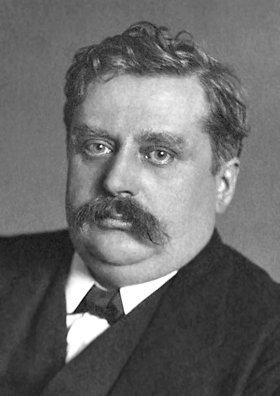
\includegraphics[width=\linewidth]{images/book3/werner.jpg}
\end{minipage}\hfill
\begin{minipage}[t]{0.74\linewidth}
\vspace{0pt}
Alfred Werner proposed in 1893 that a metal has, besides its valence, a
coordination number of groups held directly around it, and that cobalt(III) holds
six at the corners of an octahedron. He then predicted how many isomers each
formula should have and spent twenty years preparing them; in 1911 he resolved a
cobalt complex into its two enantiomers, proving that chirality does not require a
carbon atom. He received the Nobel Prize in Chemistry in 1913. (Portrait, Les Prix
Nobel, 1914, public domain, Wikimedia Commons.)
\end{minipage}
\end{history}

\section{Exercises}

\begin{exercise}[$\star$]\label{exo:b2:coordination-complexes:1}
Give the $d^n$ configuration of \ce{Ti^3+}, \ce{V^3+}, \ce{Cr^3+}, \ce{Mn^2+}, \ce{Fe^3+},
\ce{Co^2+}, \ce{Ni^2+} and \ce{Zn^2+}.
\end{exercise}

\begin{exercise}[$\star$]\label{exo:b2:coordination-complexes:2}
Give the \omterm{def:b2:coordination-complexes:denticity}{denticity} of water, ethane-1,2-diamine, the ethanedioate ion, edta and the
thiocyanate ion, and say which is ambidentate.
\end{exercise}

\begin{exercise}[$\star$]\label{exo:b2:coordination-complexes:3}
Name \ce{[Cu(NH3)4]SO4}, \ce{K3[Fe(CN)6]}, \ce{[CoCl2(NH3)4]Cl} and
\ce{[Ni(CO)4]}.
\end{exercise}

\begin{exercise}[$\star$]\label{exo:b2:coordination-complexes:4}
Predict the geometry of \ce{[Ag(NH3)2]+}, \ce{[CoCl4]^2-}, \ce{[PtCl4]^2-} and
\ce{[Fe(H2O)6]^2+}.
\end{exercise}

\begin{exercise}[$\star\star$]\label{exo:b2:coordination-complexes:5}
How many isomers does square-planar \ce{[PtCl2(NH3)2]} have? Draw them. (One of them,
cisplatin, is an anticancer drug.)
\end{exercise}

\begin{exercise}[$\star\star$]\label{exo:b2:coordination-complexes:6}
Count the valence electrons of \ce{Cr(CO)6}, \ce{Fe(CO)5}, \ce{Ni(CO)4},
\ce{V(CO)6} and \ce{Mn2(CO)10}. Which one breaks the rule, and how does it behave?
\end{exercise}

\begin{exercise}[$\star\star$]\label{exo:b2:coordination-complexes:7}
Count the valence electrons of ferrocene and of cobaltocene \ce{Co(C5H5)2}. Which is
easily oxidised, and to what?
\end{exercise}

\begin{exercise}[$\star\star$]\label{exo:b2:coordination-complexes:8}
The nickel(II) complex of edta has $\log_{10}K = 20.5$, far above that of complexes in
which nickel binds six separate nitrogen or oxygen donors. Explain this chelate effect
in terms of the number of particles released when the chelate replaces six water
molecules.
% ledger: logb:Ni-edta
\end{exercise}

\begin{exercise}[$\star\star$]\label{exo:b2:coordination-complexes:9}
Draw the two \omterm{def:b2:coordination-complexes:isomers}{linkage isomers} of \ce{[Co(NO2)(NH3)5]^2+}.
\end{exercise}

\begin{exercise}[$\star\star\star$]\label{exo:b2:coordination-complexes:10}
How many stereoisomers does \ce{[CoCl2(en)2]+} have? Which are chiral?
\end{exercise}

\begin{exercise}[$\star\star\star$]\label{exo:b2:coordination-complexes:11}
For $\mathrm{MA_4B_2}$, count the isomers predicted by a planar hexagon and by a trigonal
prism of six ligands, and explain how the number of isomers found decides between the
geometries.
\end{exercise}

\begin{exercise}[$\star\star\star$]\label{exo:b2:coordination-complexes:12}
Count the valence electrons of \ce{[RhCl(PPh3)3]} and of \ce{[IrH(CO)(PPh3)3]}
(\ce{PPh3} a two-electron donor, \ce{H-} as hydride). Which one could take up two more
ligands?
\end{exercise}

\section{Problem: Werner's Cobalt Ammines}

\begin{problem}[{Weekend problem --- four cobalt(III) chloride ammines and the chloride
they release, their formulas in brackets, the two isomers of the tetraammine and what
they prove about the geometry, and the optical activity of a tris-chelate}]
\label{pb:b2:coordination-complexes:1}
Data: four compounds A \ce{CoCl3.6NH3} (orange-yellow), B \ce{CoCl3.5NH3}
(purple), C and D \ce{CoCl3.4NH3} (green and violet). With excess silver nitrate,
one mole of A precipitates 3 mol of \ce{AgCl}, B 2 mol, C and D 1 mol each. Molar
conductivities show 4, 3, 2 and 2 ions per formula unit.

\medskip
\noindent\textbf{Part I --- Chloride and ions.}
\begin{enumerate}
  \item Which chlorides react at once with silver ions?
  \item How many chlorides are bound to cobalt in each compound?
  \item Check the numbers of ions against the conductivities.
  \item What is the oxidation number of cobalt in all four?
  \item What is its $d^n$ configuration?
  \item What total number of ligands does cobalt hold in each compound?
\end{enumerate}

\medskip
\noindent\textbf{Part II --- Formulas and names.}
\begin{enumerate}[resume]
  \item Write A, B, C and D with square brackets.
  \item Name A and B.
  \item Name the cation of C and D.
  \item What kind of isomers are C and D?
  \item What would a compound \ce{CoCl3.3NH3} be, and how many ions would it give?
  \item How many isomers would that compound have in an octahedron?
\end{enumerate}

\medskip
\noindent\textbf{Part III --- The geometry.}
\begin{enumerate}[resume]
  \item Draw cis and trans \ce{[CoCl2(NH3)4]+} in an octahedron.
  \item Count the isomers of \ce{[CoCl2(NH3)4]+} predicted for six ligands at the
        corners of a planar hexagon.
  \item Count those predicted for a trigonal prism.
  \item Werner never found more than two. What does it prove?
  \item Is the proof complete? What would a third isomer have meant?
  \item Which of C and D is cis, knowing that the cis isomer can be converted into a
        chelate with ethanedioate and the trans cannot?
\end{enumerate}

\medskip
\noindent\textbf{Part IV --- Optical activity.}
\begin{enumerate}[resume]
  \item Draw \ce{[Co(en)3]^3+}.
  \item Does it have a mirror plane? A centre of inversion?
  \item How many stereoisomers does it have?
  \item What does the resolution of such a cation into enantiomers prove?
  \item Is \ce{[CoCl2(en)2]+} chiral in its cis form? In its trans form?
  \item Why did Werner's resolution of a complex containing no carbon at all matter?
  \item State the number of isomers of \ce{[CoCl2(NH3)4]+} predicted by the octahedron,
        and by the planar hexagon and the trigonal prism.
\end{enumerate}
\end{problem}
